\documentclass[12pt]{article}

\usepackage[utf8]{inputenc}
\usepackage{latexsym,amsfonts,amssymb,amsthm,amsmath}

\setlength{\parindent}{0in}
\setlength{\oddsidemargin}{0in}
\setlength{\textwidth}{6.5in}
\setlength{\textheight}{8.8in}
\setlength{\topmargin}{0in}
\setlength{\headheight}{18pt}
\usepackage{graphicx} % Required for inserting images
\usepackage{enumitem}
\usepackage{listings}
\lstset{
    basicstyle=\scriptsize\ttfamily,
    breaklines=true,
    frame=single
}

\usepackage{xcolor}

\usepackage{booktabs}

\usepackage{tikz}
\usepackage{pgfplots}
\pgfplotsset{compat=1.18}

\usepackage[toc]{appendix}

\title{Econometría 2502 - Taller 2}
\author{Rafael Marulanda y Lorena Toro}
\date{27 de setiembre de 2025}

\begin{document}

\maketitle

\section{Ejercicio sobre la base de datos \texttt{wage1}}

Descargue la base de datos \texttt{wage1}.

\begin{enumerate}[label=\alph*)]
    \item Calcule estadísticas descriptivas de \texttt{wage}, \texttt{educ}, \texttt{exper}, \texttt{tenure} y \texttt{numdep}. Muestre sus resultados. Calcule el histograma de frecuencias de cada una de las variables. Interprete sus resultados.
    
    \item Tabule y calcule las estadísticas descriptivas de las variables \texttt{nonwhite}, \texttt{female} y \texttt{married}. Interprete sus resultados.
    
    \item Calcule el número de mujeres no blancas en la muestra.
    
    \item Calcule el número de hombres blancos y casados de la muestra.
    
    \item Calcule el número de mujeres blancas y solteras en la muestra.
    
    \item Calcule la covarianza y la correlación entre \texttt{wage}, \texttt{educ}, \texttt{exper}, \texttt{tenure} y \texttt{numdep}.
\end{enumerate}

\subsection*{a) Estadísticas Descriptivas}

\subsubsection*{Salida de Stata de la parte a}

\lstinputlisting[label=lst:hwrk-0201-a]{Outputs/ecnm-2502-outp-hwrk-0201-a.txt}

\subsubsection*{Resumen de las Distribuciones de Variables}

La Tabla \ref{tab:descriptive_statistics} proporciona las estadísticas resumen para las variables continuas: salarios por hora, años de educación, experiencia en el mercado laboral, antigüedad en el empleo y número de dependientes económicos.

\begin{table}[htbp]\centering
\def\sym#1{\ifmmode^{#1}\else\(^{#1}\)\fi}
\caption{Descriptive Statistics}
\label{tab:0201-descriptive_statistics}
\begin{tabular}{l*{1}{ccccc}}
\toprule
                    &\multicolumn{5}{c}{(1)}                                         \\
                    &\multicolumn{5}{c}{}                                            \\
                    &        mean&          sd&         min&         max&       count\\
\midrule
average hourly earnings&        5.90&        3.69&        0.53&       24.98&      526.00\\
years of education  &       12.56&        2.77&        0.00&       18.00&      526.00\\
years potential experience&       17.02&       13.57&        1.00&       51.00&      526.00\\
years with current employer&        5.10&        7.22&        0.00&       44.00&      526.00\\
number of dependents&        1.04&        1.26&        0.00&        6.00&      526.00\\
\midrule
Observations        &         526&            &            &            &            \\
\bottomrule
\end{tabular}
\end{table}


\subsubsection*{Análisis de la Distribución Salarial}

La variable de salario, medida en dólares por hora, presenta una media de \$5.90 con una desviación estándar de \$3.69, como se muestra en la Tabla \ref{tab:0201-descriptive_statistics}. La distribución muestra un sesgo positivo pronunciado, evidenciado por la diferencia entre la media (\$5.90) y la mediana (\$4.65). Este sesgo hacia la derecha indica que mientras la mayoría de los trabajadores perciben salarios modestos, una pequeña proporción de trabajadores con altos ingresos influye significativamente en el promedio hacia arriba.

La Figura \ref{fig:hist_wage} ilustra la distribución de frecuencias de los salarios, revelando una concentración de observaciones en el rango de \$2-\$6 con una cola larga hacia la derecha que se extiende hasta el valor máximo de \$24.98. Este patrón se alinea con los fenómenos de desigualdad salarial bien documentados en la literatura de economía laboral, donde las diferencias en capital humano y la segmentación del mercado laboral contribuyen a la dispersión de ingresos.

\begin{figure}[h!]
\centering
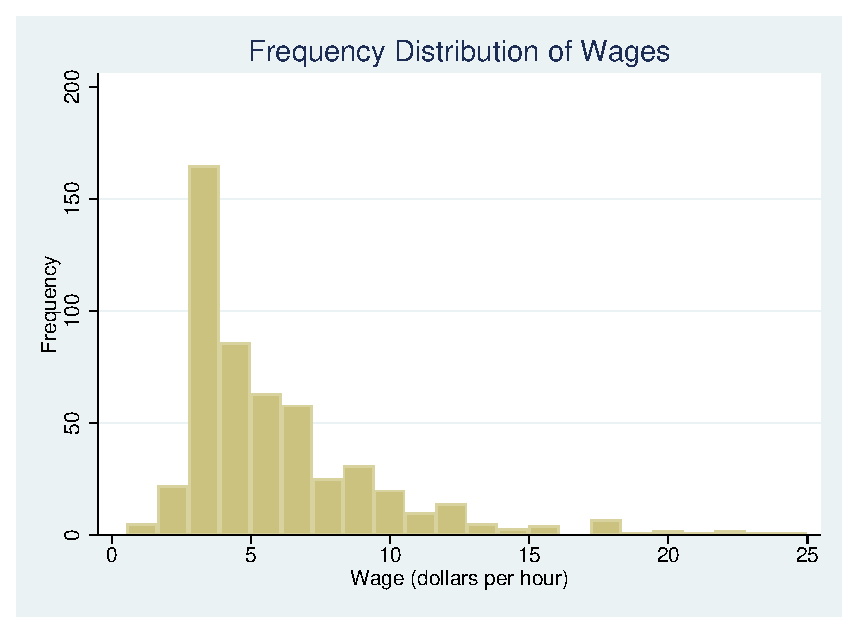
\includegraphics[width=0.8\textwidth]{Figures/0201-hist_wage.eps}
\caption{Distribución de Frecuencias de Salarios}
\label{fig:hist_wage}
\end{figure}

\subsubsection*{Patrones de Logro Educativo}

La variable de educación presenta una media de 12.56 años y una desviación estándar de 2.77 años. La Figura \ref{fig:hist_educ} revela una concentración notable exactamente en 12 años de educación, correspondiente a la finalización de la educación secundaria. Este pico modal, que abarca aproximadamente 200 observaciones, domina la distribución y sugiere que la fuerza laboral consiste principalmente en graduados de secundaria.

La desviación estándar relativamente modesta indica heterogeneidad educativa limitada dentro de la muestra. El rango se extiende desde 0 hasta 18 años, capturando individuos sin educación formal hasta aquellos con títulos de posgrado. Sin embargo, la concentración alrededor de la finalización de la educación secundaria sugiere que esta muestra puede representar un segmento particular del mercado laboral, posiblemente trabajadores del sector manufacturero o de servicios.

\begin{figure}[h!]
\centering
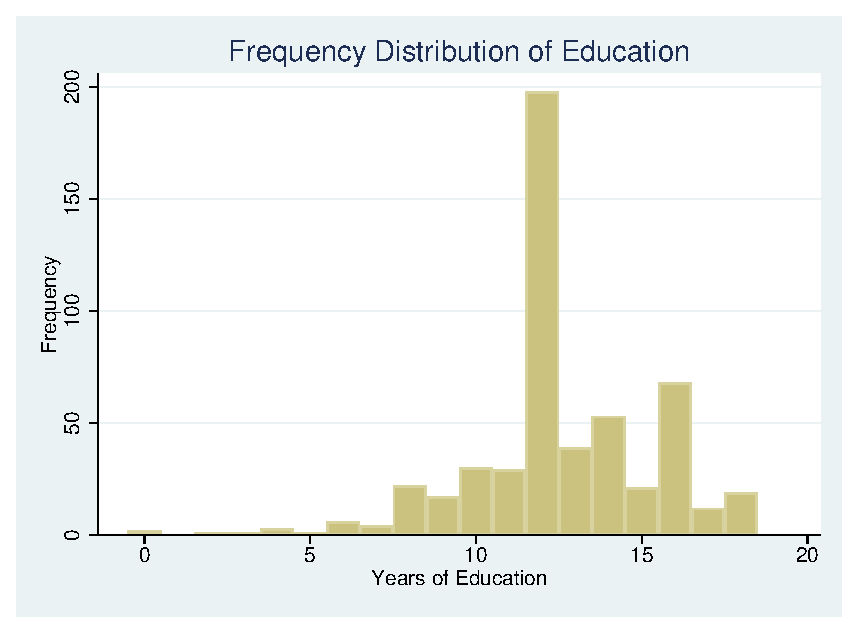
\includegraphics[width=0.8\textwidth]{Figures/0201-hist_educ.eps}
\caption{Distribución de Frecuencias de Años de Educación}
\label{fig:hist_educ}
\end{figure}

\subsubsection*{Distribución de Experiencia y Dinámica Profesional}

La experiencia en el mercado laboral, con una media de 17.02 años y una desviación estándar de 13.57 años, muestra una variabilidad considerable a través de la muestra. La Figura \ref{fig:hist_exper} muestra una distribución con sesgo positivo, con la frecuencia más alta ocurriendo entre trabajadores con niveles de experiencia relativamente bajos (1-10 años), seguida de una disminución gradual en frecuencia a medida que aumenta la experiencia.

La mediana de experiencia de 13.5 años cae por debajo de la media, confirmando el sesgo positivo de la distribución. El valor máximo de 51 años indica la presencia de trabajadores acercándose a la edad de jubilación, mientras que el mínimo de 1 año sugiere recién ingresados al mercado laboral. Este amplio rango refleja una fuerza laboral que abarca múltiples etapas profesionales, desde trabajadores en inicio de carrera hasta aquellos con participación extensa en el mercado laboral.

\begin{figure}[h!]
\centering
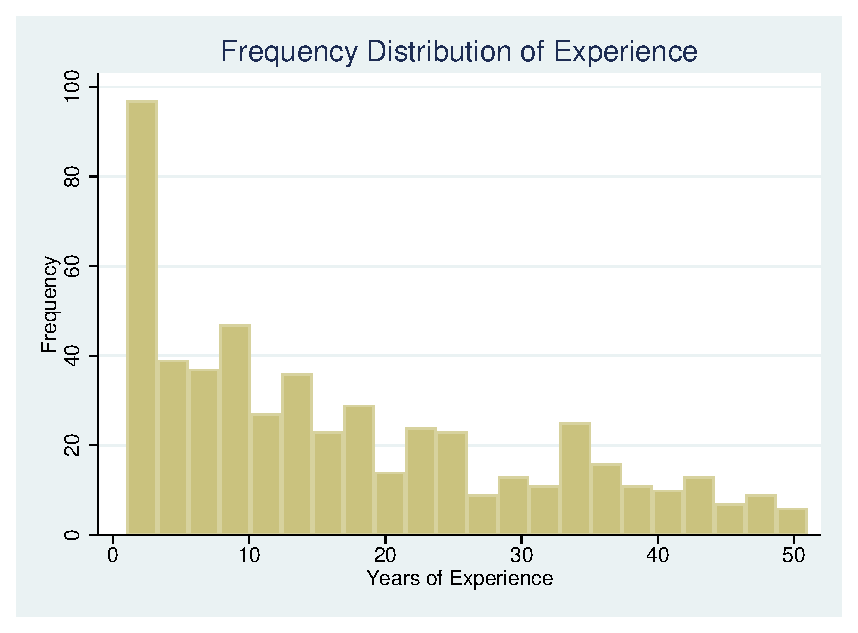
\includegraphics[width=0.8\textwidth]{Figures/0201-hist_expr.eps}
\caption{Distribución de Frecuencias de Años de Experiencia}
\label{fig:hist_exper}
\end{figure}

\subsubsection*{Antigüedad Laboral y Estabilidad en el Empleo}

La variable de antigüedad presenta las características distribucionales más extremas entre todas las variables examinadas. Con una media de 5.10 años pero una mediana de solo 2 años, la distribución exhibe un sesgo positivo severo. La Figura \ref{fig:hist_tenure} revela que aproximadamente 220 trabajadores (~42\% de la muestra) reportan cero antigüedad con su empleador actual, sugiriendo tasas altas de rotación laboral.

La desviación estándar de 7.22 años excede la media, indicando variabilidad extrema en los patrones de vinculación laboral. Mientras que la mayoría de los trabajadores demuestran antigüedad limitada con su empleador actual, el valor máximo de 44 años revela la presencia de trabajadores con estabilidad laboral excepcional.

\begin{figure}[h!]
\centering
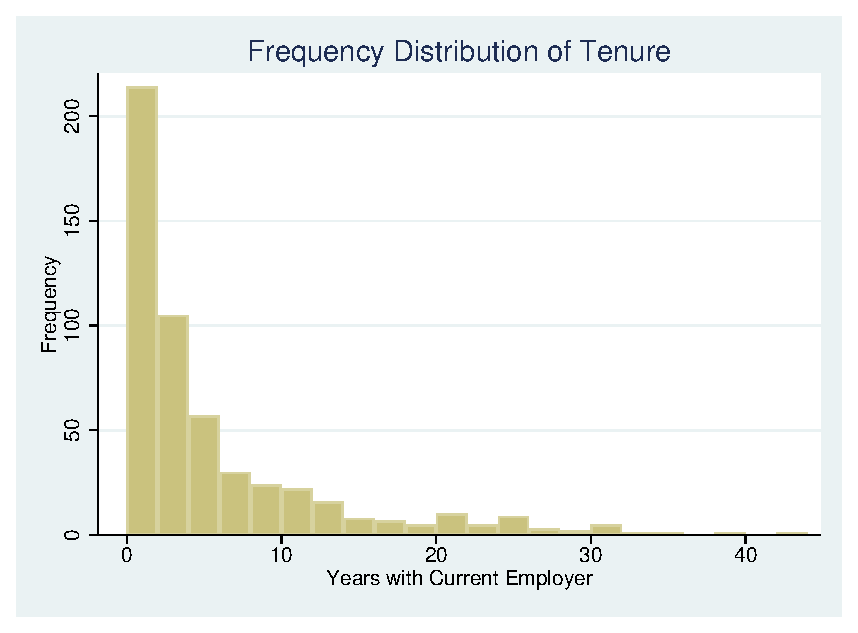
\includegraphics[width=0.8\textwidth]{Figures/0201-hist_tenr.eps}
\caption{Distribución de Frecuencias de Años de Antigüedad}
\label{fig:hist_tenure}
\end{figure}

\subsubsection*{Composición del Hogar y Dependientes}

La variable del número de dependientes muestra una media de 1.04 con una desviación estándar de 1.26. La distribución se concentra fuertemente en valores bajos, con la mediana en 1 dependiente. El máximo de 6 dependientes ocurre raramente en la muestra, indicando que las familias grandes son poco comunes entre esta fuerza laboral.

\begin{figure}[h!]
\centering
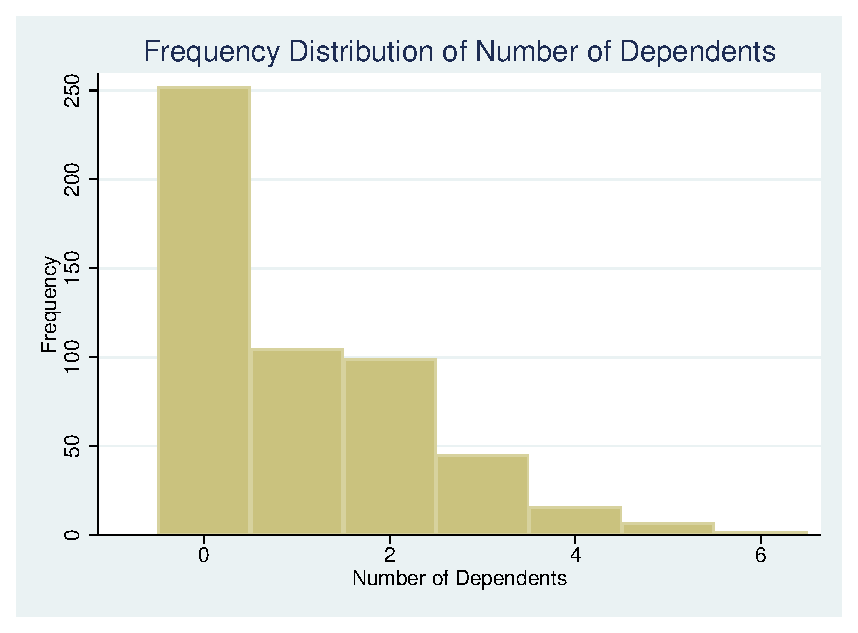
\includegraphics[width=0.8\textwidth]{Figures/0201-hist_numd.eps}
\caption{Distribución de Frecuencias de Número de Dependientes}
\label{fig:hist_numdep}
\end{figure}

\subsubsection*{Interpretación general}

El análisis descriptivo revela varios patrones importantes que caracterizan esta muestra del mercado laboral. Primero, la pronunciada desigualdad salarial, evidenciada por la distribución sesgada de salarios. Segundo, la concentración del logro educativo en el nivel de secundaria sugiere una fuerza laboral posicionada en el medio de la distribución de habilidades, no dominada ni por graduados universitarios ni por trabajadores sin educación básica.

La desconexión entre la experiencia promedio (17 años) y la antigüedad promedio (5 años) indica movilidad laboral sustancial a lo largo de las carreras de los trabajadores. Tal movilidad puede reflejar tanto cambios de trabajo voluntarios para el avance profesional como separaciones involuntarias debido a condiciones económicas.

El número promedio relativamente bajo de dependientes, junto con la proporción sustancial de trabajadores sin dependientes, puede indicar una demografía de fuerza laboral más joven.

Estas características distribucionales muestran colectivamente un cuadro de un segmento del mercado laboral caracterizado por niveles de habilidad moderados, dispersión salarial significativa, alta movilidad laboral y estructuras familiares variadas.

\subsection*{b) Análisis de variables categóricas}

\subsubsection*{Salida de Stata de la parte b)}

\lstinputlisting[label=lst:hwrk-0201-b]{Outputs/ecnm-2502-outp-hwrk-0201-b.txt}

\subsubsection*{Distribución y Características de las Variables Binarias}

El análisis de las variables categóricas \texttt{nonwhite}, \texttt{female} y \texttt{married} proporciona información fundamental sobre la composición demográfica de la muestra. La Tabla \ref{tab:0201-categorical_summary} presenta un resumen de estas variables binarias, mientras que las Tablas \ref{tab:0201-nonwhite_frequency}, \ref{tab:0201-female_frequency} y \ref{tab:0201-married_frequency} detallan sus distribuciones individuales.

\begin{table}[htbp]\centering
\def\sym#1{\ifmmode^{#1}\else\(^{#1}\)\fi}
\caption{Summary of Categorical Variables}\label{tab:0201-categorical_summary}
\begin{tabular}{l*{1}{cc}}
\toprule
            &\multicolumn{2}{c}{(1)}  \\
            &\multicolumn{2}{c}{}     \\
            &        mean&       count\\
\midrule
nonwhite    &       0.103&         526\\
female      &       0.479&         526\\
married     &       0.608&         526\\
\midrule
\(N\)       &         526&            \\
\bottomrule
\multicolumn{3}{l}{\footnotesize Proportions and sample sizes shown}\\
\end{tabular}
\end{table}

\begin{table}[htbp]\centering
\def\sym#1{\ifmmode^{#1}\else\(^{#1}\)\fi}
\caption{Distribution by Race}
\begin{tabular}{l*{1}{c}}
\toprule
            &\multicolumn{1}{c}{(1)}\\
            &\multicolumn{1}{c}{nonwhite}\\
            &       b/pct\\
\midrule
0           &         472\\
            &        89.7\\
1           &          54\\
            &        10.3\\
Total       &         526\\
            &       100.0\\
\midrule
\(N\)       &         526\\
\bottomrule
\multicolumn{2}{l}{\footnotesize Frequency and percentage shown}\\
\end{tabular}
\end{table}

\begin{table}[htbp]\centering
\def\sym#1{\ifmmode^{#1}\else\(^{#1}\)\fi}
\caption{Distribution by Gender}\label{tab:0201-female_frequency}
\begin{tabular}{l*{1}{c}}
\toprule
            &\multicolumn{1}{c}{(1)}\\
            &\multicolumn{1}{c}{female}\\
            &       b/pct\\
\midrule
0           &         274\\
            &        52.1\\
1           &         252\\
            &        47.9\\
Total       &         526\\
            &       100.0\\
\midrule
\(N\)       &         526\\
\bottomrule
\multicolumn{2}{l}{\footnotesize Frequency and percentage shown}\\
\end{tabular}
\end{table}

\begin{table}[htbp]\centering
\def\sym#1{\ifmmode^{#1}\else\(^{#1}\)\fi}
\caption{Distribution by Marital Status}\label{tab:0201-married_frequency}
\begin{tabular}{l*{1}{c}}
\toprule
            &\multicolumn{1}{c}{(1)}\\
            &\multicolumn{1}{c}{married}\\
            &       b/pct\\
\midrule
0           &         206\\
            &        39.2\\
1           &         320\\
            &        60.8\\
Total       &         526\\
            &       100.0\\
\midrule
\(N\)       &         526\\
\bottomrule
\multicolumn{2}{l}{\footnotesize Frequency and percentage shown}\\
\end{tabular}
\end{table}


\subsubsection*{Composición Racial}

La variable \texttt{nonwhite} revela una muestra predominantemente blanca, con solo el 10.27\% (54 trabajadores) identificados como no blancos y el 89.73\% (472 trabajadores) como blancos.

La Tabla \ref{tab:0201-descriptives_by_race} presenta diferencias en las características económicas por grupo racial. Los trabajadores blancos perciben salarios promedio de \$5.94 por hora, mientras que los no blancos reciben \$5.48, una diferencia de \$0.47 o aproximadamente 8\% menos. Los trabajadores no blancos presentan menor logro educativo promedio (11.87 vs 12.64 años), equivalente a casi un año menos de escolaridad. Esta diferencia educativa podría explicar parcialmente la disparidad salarial observada, aunque no puede descartarse la presencia de discriminación laboral.

\begin{table}[htbp]\centering
\def\sym#1{\ifmmode^{#1}\else\(^{#1}\)\fi}
\caption{Descriptive Statistics by Race}
\begin{tabular}{l*{1}{ccc}}
\toprule
            &\multicolumn{3}{c}{(1)}               \\
            &\multicolumn{3}{c}{White}             \\
            &        mean&          sd&       count\\
\midrule
0           &            &            &            \\
wage        &        5.94&        3.75&         472\\
educ        &       12.64&        2.69&         472\\
exper       &       16.95&       13.58&         472\\
tenure      &        5.08&        7.28&         472\\
\midrule
1           &            &            &            \\
wage        &        5.48&        3.16&          54\\
educ        &       11.87&        3.32&          54\\
exper       &       17.59&       13.58&          54\\
tenure      &        5.35&        6.79&          54\\
\midrule
Total       &            &            &            \\
wage        &        5.90&        3.69&         526\\
educ        &       12.56&        2.77&         526\\
exper       &       17.02&       13.57&         526\\
tenure      &        5.10&        7.22&         526\\
\midrule
\(N\)       &         526&            &            \\
\bottomrule
\multicolumn{4}{l}{\footnotesize Standard deviations shown below means}\\
\end{tabular}
\end{table}


\subsubsection*{Distribución por Género}

La variable \texttt{female} muestra una distribución algo equilibrada con 52.09\% hombres (274 trabajadores) y 47.91\% mujeres (252 trabajadoras). Esta proporción cercana a la paridad sugiere una muestra representativa en términos de participación laboral por género para el período analizado.

Sin embargo, la Tabla \ref{tab:0201-descriptives_by_gender} revela disparidades económicas sustanciales entre géneros. Los hombres ganan en promedio \$7.10 por hora comparado con \$4.59 para las mujeres, representando una brecha salarial del 54.7\%. Esta diferencia dramática constituye la disparidad más pronunciada entre todas las variables categóricas analizadas. Las mujeres también presentan menor educación promedio (12.32 vs 12.79 años), menor experiencia laboral (16.43 vs 17.56 años), y notablemente menor antigüedad laboral (3.62 vs 6.47 años). La diferencia en antigüedad sugiere mayor rotación laboral femenina, posiblemente relacionada con interrupciones de carrera por responsabilidades familiares o discriminación en retención laboral.

\begin{table}[htbp]\centering
\def\sym#1{\ifmmode^{#1}\else\(^{#1}\)\fi}
\caption{Descriptive Statistics by Gender}\label{tab:0201-descriptives_by_gender}
\begin{tabular}{l*{1}{ccc}}
\toprule
            &\multicolumn{3}{c}{(1)}               \\
            &\multicolumn{3}{c}{Male}              \\
            &        mean&          sd&       count\\
\midrule
0           &            &            &            \\
wage        &        7.10&        4.16&         274\\
educ        &       12.79&        3.00&         274\\
exper       &       17.56&       13.50&         274\\
tenure      &        6.47&        8.37&         274\\
\midrule
1           &            &            &            \\
wage        &        4.59&        2.53&         252\\
educ        &       12.32&        2.47&         252\\
exper       &       16.43&       13.65&         252\\
tenure      &        3.62&        5.36&         252\\
\midrule
Total       &            &            &            \\
wage        &        5.90&        3.69&         526\\
educ        &       12.56&        2.77&         526\\
exper       &       17.02&       13.57&         526\\
tenure      &        5.10&        7.22&         526\\
\midrule
\(N\)       &         526&            &            \\
\bottomrule
\multicolumn{4}{l}{\footnotesize Standard deviations shown below means}\\
\end{tabular}
\end{table}


\subsubsection*{Estado Civil}

La variable \texttt{married} indica que el 60.84\% de la muestra (320 trabajadores) está casada, mientras que el 39.16\% (206 trabajadores) permanece soltera.

La Tabla \ref{tab:0201-descriptives_by_marital} revela que los trabajadores casados perciben salarios significativamente superiores (\$6.57 vs \$4.84), una prima matrimonial del 35.7\%. Los casados también exhiben mayor experiencia laboral (20.47 vs 11.66 años) y antigüedad (6.49 vs 2.95 años). Estas diferencias sugieren que el matrimonio puede estar correlacionado con mayor estabilidad laboral y acumulación de capital humano, aunque también podría reflejar efectos de selección donde individuos con mejores perspectivas económicas tienen mayor probabilidad de casarse.

\begin{table}[htbp]\centering
\def\sym#1{\ifmmode^{#1}\else\(^{#1}\)\fi}
\caption{Descriptive Statistics by Marital Status}\label{tab:0201-descriptives_by_marital}
\begin{tabular}{l*{1}{ccc}}
\toprule
            &\multicolumn{3}{c}{(1)}               \\
            &\multicolumn{3}{c}{Single}            \\
            &        mean&          sd&       count\\
\midrule
0           &            &            &            \\
wage        &        4.84&        2.89&         206\\
educ        &       12.33&        2.74&         206\\
exper       &       11.66&       13.10&         206\\
tenure      &        2.95&        5.31&         206\\
\midrule
1           &            &            &            \\
wage        &        6.57&        3.99&         320\\
educ        &       12.72&        2.78&         320\\
exper       &       20.47&       12.74&         320\\
tenure      &        6.49&        7.93&         320\\
\midrule
Total       &            &            &            \\
wage        &        5.90&        3.69&         526\\
educ        &       12.56&        2.77&         526\\
exper       &       17.02&       13.57&         526\\
tenure      &        5.10&        7.22&         526\\
\midrule
\(N\)       &         526&            &            \\
\bottomrule
\multicolumn{4}{l}{\footnotesize Standard deviations shown below means}\\
\end{tabular}
\end{table}


\subsubsection*{Raza y Género}

La distribución por género es similar entre grupos raciales: 51.91\% de los trabajadores blancos son hombres comparado con 53.70\% entre no blancos. Esta similitud sugiere que no existe segregación ocupacional significativa por género dentro de grupos raciales en esta muestra. Tablas \ref{tab:0201-crosstab_race_gender}

\begin{table}[htbp]\centering
\def\sym#1{\ifmmode^{#1}\else\(^{#1}\)\fi}
\caption{Cross-tabulation: Race by Gender}\label{tab:0201-crosstab_race_gender}
\begin{tabular}{l*{1}{c}}
\toprule
            &\multicolumn{1}{c}{(1)}\\
            &\multicolumn{1}{c}{}\\
            &           b\\
\midrule
0           &            \\
0           &         245\\
1           &          29\\
Total       &         274\\
\midrule
1           &            \\
0           &         227\\
1           &          25\\
Total       &         252\\
\midrule
Total       &            \\
0           &         472\\
1           &          54\\
Total       &         526\\
\midrule
\(N\)       &         526\\
\bottomrule
\multicolumn{2}{l}{\footnotesize Cell frequencies shown}\\
\end{tabular}
\end{table}


\subsubsection*{Raza y Estado Civil}

Como muestra la Tabla \ref{tab:0201-crosstab_race_married} los trabajadores blancos muestran mayor tasa de matrimonio (61.86\%) comparado con los no blancos (51.85\%). Esta diferencia de 10 puntos porcentuales podría reflejar factores socioeconómicos que afectan las decisiones matrimoniales, incluyendo estabilidad económica y normas culturales diferenciadas.

\begin{table}[htbp]\centering
\def\sym#1{\ifmmode^{#1}\else\(^{#1}\)\fi}
\caption{Cross-tabulation: Race by Marital Status}\label{tab:0201-crosstab_race_married}
\begin{tabular}{l*{1}{c}}
\toprule
            &\multicolumn{1}{c}{(1)}\\
            &\multicolumn{1}{c}{}\\
            &           b\\
\midrule
0           &            \\
0           &         180\\
1           &          26\\
Total       &         206\\
\midrule
1           &            \\
0           &         292\\
1           &          28\\
Total       &         320\\
\midrule
Total       &            \\
0           &         472\\
1           &          54\\
Total       &         526\\
\midrule
\(N\)       &         526\\
\bottomrule
\multicolumn{2}{l}{\footnotesize Cell frequencies shown}\\
\end{tabular}
\end{table}


\subsubsection*{Género y Estado Civil}

La Tabla \ref{tab:0201-crosstab_gender_married} revela patrones matrimoniales marcadamente diferentes por género. El 68.61\% de los hombres están casados versus solo 52.38\% de las mujeres. Esta disparidad sugiere que las mujeres solteras tienen mayor participación laboral que los hombres solteros, consistente con teorías de especialización familiar donde las mujeres casadas enfrentan mayores barreras para la participación laboral.

\begin{table}[htbp]\centering
\def\sym#1{\ifmmode^{#1}\else\(^{#1}\)\fi}
\caption{Cross-tabulation: Gender by Marital Status}\label{tab:0201-crosstab_gender_married}
\begin{tabular}{l*{1}{c}}
\toprule
            &\multicolumn{1}{c}{(1)}\\
            &\multicolumn{1}{c}{}\\
            &           b\\
\midrule
0           &            \\
0           &          86\\
1           &         120\\
Total       &         206\\
\midrule
1           &            \\
0           &         188\\
1           &         132\\
Total       &         320\\
\midrule
Total       &            \\
0           &         274\\
1           &         252\\
Total       &         526\\
\midrule
\(N\)       &         526\\
\bottomrule
\multicolumn{2}{l}{\footnotesize Cell frequencies shown}\\
\end{tabular}
\end{table}


\subsubsection*{Interpretación General}

Los resultados revelan segmentación significativa del mercado laboral según características demográficas. Las brechas salariales observadas—8\% por raza, 54.7\% por género, y 35.7\% por estado civil—sugieren que factores más allá del capital humano influyen en la determinación salarial. La intersección de estas características probablemente amplifica las desventajas: una mujer no blanca soltera enfrenta múltiples penalizaciones salariales acumulativas.

La menor antigüedad laboral de mujeres y trabajadores no blancos indica menor acumulación de capital humano específico a la empresa, y potencialmente menor acceso a promociones internas. Estos patrones sugieren la necesidad de políticas laborales que aborden las brechas salariales directas y las barreras estructurales que impiden la acumulación de experiencia y antigüedad en grupos desfavorecidos.

El análisis también sugiere que el matrimonio funciona como un marcador de estabilidad económica y laboral, aunque la causalidad permanece ambigua. Los trabajadores casados podrían recibir primas salariales debido a mayor productividad percibida, discriminación estadística favorable, o simplemente porque individuos económicamente exitosos tienen mayor probabilidad de casarse y permanecer casados.



\subsection*{c) Número de mujeres no blancas}

El número de mujeres no blancas en la muestra es 25.

\subsubsection*{Salida de Stata de la parte c)}

%\lstinputlisting[label=lst:hwrk-0201-c]{Outputs/ecnm-2502-outp-hwrk-0201-c.txt}

\subsection*{d) Número de hombres blancos y casados}

El número de hombres blancos y casados en la muestra es 168.

\subsubsection*{Salida de Stata de la parte d)}

%\lstinputlisting[label=lst:hwrk-0201-d]{Outputs/ecnm-2502-outp-hwrk-0201-d.txt}

\subsection*{e) Número de mujeres blancas y solteras}

El número de mujeres blancas y solteras en la muestra es 103.

\subsubsection*{Salida de Stata de la parte e)}

%\lstinputlisting[label=lst:hwrk-0201-e]{Outputs/ecnm-2502-outp-hwrk-0201-e.txt}

\subsection*{f) Cálculo de la covarianza y correlación}

Los cálculos de varianza y correlación entre \texttt{wage}, \texttt{educ}, \texttt{exper}, \texttt{tenure} y \texttt{numdep} se resumen en la tabla XX construida con los datos de la salida de Stata de la parte f). 

\subsubsection*{Salida de Stata de la parte f)}

%\lstinputlisting[label=lst:hwrk-0201-f]{Outputs/ecnm-2502-outp-hwrk-0201-f.txt}

\section{Regresión lineal simple: predicción de ventas}

Una pequeña empresa contrata a un consultor para predecir el valor de las ventas semanales de su producto si el gasto en publicidad semanal aumenta a \$750. 
El consultor lleva un registro de cuánto gastó la empresa en publicidad por semana y las ventas semanales correspondientes durante los últimos seis meses. 

El consultor escribe: 
\begin{quote}
``Durante los últimos seis meses, el gasto semanal promedio en publicidad ha sido de \$500 y las ventas semanales promedio han sido de \$10{,}000. 
Según los resultados de una regresión lineal simple, predigo que las ventas serán de \$12{,}000 si se gastan \$750 por semana en publicidad''.
\end{quote}

\begin{enumerate}[label=\alph*)]
    \item ¿Cuál es la regresión simple estimada utilizada por el consultor para hacer esta predicción?
    \item Dibuje un gráfico de la línea de regresión estimada. 
    Busque los valores semanales promedio en el gráfico.
\end{enumerate}

\subsection*{a) Regresión Simple Estimada}

El modelo de regresión lineal simple poblacional se especifica como:
$$
\text{Ventas} = \beta_0 + \beta_1 \cdot \text{Publicidad} + u
$$
Donde:
\begin{itemize}
    \item \textit{Ventas} es la variable dependiente ($y$).
    \item \textit{Publicidad} es la variable independiente ($x$).
    \item $\beta_0$ es el intercepto.
    \item $\beta_1$ es la pendiente.
    \item $u$ es el término de error.
\end{itemize}

El consultor utiliza un modelo de regresión lineal. La ecuación de esta línea estimada es:
$$
\hat{\text{Ventas}} = \hat{\beta}_0 + \hat{\beta}_1 \cdot \text{Publicidad}
$$

Para encontrar los valores de los estimadores, se usa la información dada:
\begin{itemize}
    \item El gasto semanal promedio en publicidad ($\bar{x}$) es de \$500.
    \item Las ventas semanales promedio ($\bar{y}$) son de \$10,000.
    \item Una predicción específica: cuando el gasto en publicidad ($x_p$) es 750, las ventas predichas ($\hat{y}_p$) son \$12,000.
\end{itemize}

Una propiedad de la regresión lineal es que la línea de regresión siempre pasa por el punto de las medias ($\bar{x}, \bar{y}$). Por lo tanto, este punto debe satisfacer la ecuación de regresión:
\begin{equation*}
\text{Ecuación 1: } \bar{y} = \hat{\beta}_0 + \hat{\beta}_1 \bar{x} \implies 10,000 = \hat{\beta}_0 + \hat{\beta}_1(500)
\end{equation*}

Además, se sabe que el punto de la predicción (750, 12,000) también se encuentra sobre la línea de regresión estimada:
\begin{equation*}
\text{Ecuación 2: } 12,000 = \hat{\beta}_0 + \hat{\beta}_1(750)
\end{equation*}

Ahora se tiene un sistema de dos ecuaciones lineales con dos incógnitas ($\hat{\beta}_0$ y $\hat{\beta}_1$). Se resuelve restando la Ecuación 1 de la Ecuación 2:
\begin{align*}
(12,000 - 10,000) &= (\hat{\beta}_0 + 750\hat{\beta}_1) - (\hat{\beta}_0 + 500\hat{\beta}_1) \\
2,000 &= 250\hat{\beta}_1
\end{align*}

Despejando $\hat{\beta}_1$:
$$
\hat{\beta}_1 = \frac{2,000}{250} = 8
$$
Esta pendiente ($\hat{\beta}_1 = 8$) indica el efecto marginal. Significa que, por cada dólar adicional gastado en publicidad, las ventas semanales aumentarán en \$8.\\

Se substituye el valor de $\hat{\beta}_1$ en la Ecuación 1 para encontrar el intercepto ($\hat{\beta}_0$):
\begin{align*}
10,000 &= \hat{\beta}_0 + 8(500) \\
10,000 &= \hat{\beta}_0 + 4,000 \\
\hat{\beta}_0 &= 10,000 - 4,000 = 6,000
\end{align*}
El intercepto ($\hat{\beta}_0 = 6,000$) es el valor predicho de las ventas semanales si el gasto en publicidad es cero.\\

Por lo tanto, la regresión simple estimada utilizada por el consultor es:
$$
\hat{\text{Ventas}} = 6,000 + 8 \cdot \text{Publicidad}
$$

\subsection*{b) Gráfico de la línea de Regresión Estimada}

Una línea se define con dos puntos, entonces usando los puntos dados se define esta. 
El eje horizontal ($X$) representa el \emph{Gasto en Publicidad} y el eje vertical ($Y$) representa las \emph{Ventas Semanales}.\\

Los puntos clave en esta línea son:

\begin{itemize}
    \item El intercepto en $Y$: $(0,\,6000)$
    \item El punto de las medias: $(\bar{x},\bar{y}) = (500,\,10000)$
    \item El punto de predicción: $(750,\,12000)$
\end{itemize}

\begin{figure}[ht]
    \centering
    \begin{tikzpicture}
        \begin{axis}[
            width=12cm,
            height=8cm,
            xlabel={Gasto en Publicidad (\$)},
            ylabel={Ventas Semanales (\$)},
            xmin=0, xmax=1200,
            ymin=0, ymax=15000,
            grid=both,
            grid style={dashed,gray!30},
            axis lines=left,
            enlargelimits=false,
            legend pos=south east,
            % ticks
            xtick={0,200,400,600,800,1000,1200},
            ytick={0,2000,4000,6000,8000,10000,12000,14000}
        ]
            % regression line: y = 6000 + 8*x
            \addplot[
                domain=0:1200,
                samples=2,
                thick
            ] {6000 + 8*x};
            \addlegendentry{Línea de regresión $\hat{y}=6000+8x$}

            % intercept point (0,6000)
            \addplot[
                only marks,
                mark=*,
                mark size=2.5pt
            ] coordinates {(0,6000)};
            \addlegendentry{Intercepto $(0,6000)$}

            % mean point (500,10000)
            \addplot[
                only marks,
                mark=square*,
                mark size=3.0pt
            ] coordinates {(500,10000)};
            \addlegendentry{Punto de las medias $(500,10000)$}

            % prediction point (750,12000)
            \addplot[
                only marks,
                mark=triangle*,
                mark size=3.5pt
            ] coordinates {(750,12000)};
            \addlegendentry{Predicción $(750,12000)$}

            % Labels next to the points
            \node[pin=135:{$(0,6000)$}] at (axis cs:0,6000) {};
            \node[pin= -45:{$(\bar{x},\bar{y})=(500,10000)$}] at (axis cs:500,10000) {};
            \node[pin= 45:{$(750,12000)$}] at (axis cs:750,12000) {};
        \end{axis}
    \end{tikzpicture}
    \caption{Línea de regresión estimada y puntos clave (intercepto, medias y predicción).}
\end{figure}
 
El punto de las medias actúa como el ``centro de gravedad'' para la nube de datos a partir de la cual se estimó la regresión.

\newpage
\section{Relación entre temperatura y ventas de refrescos}

Un vendedor de gaseosas en los juegos de baseball de la Universidad de Costa Rica observa que se venden más refrescos cuanto más cálida es la temperatura en el momento del juego. Basado en 32 juegos en casa que cubren cinco años, el proveedor estima que la relación entre las ventas de refrescos y la temperatura es

\[
\hat{y} = -240 + 8x,
\]

donde $y$ es el número de refrescos que vende y $x$ la temperatura en grados Fahrenheit.

\begin{enumerate}[label=\alph*)]
    \item Interprete los parámetros estimados. ¿Tienen sentido las estimaciones? ¿Por qué o por qué no?
    \item En un día en el que se pronostique que la temperatura a la hora del juego será 80$^\circ$F, prediga cuántos refrescos venderá el vendedor.
    \item ¿Por debajo de qué temperatura son cero las ventas previstas?
    \item Dibuje un gráfico de la línea de regresión estimada.
\end{enumerate}

\subsection*{a) Interpretación de los Parámetros Estimados}

La función de regresión muestral estimada es:  

\[
\hat{y} = -240 + 8x
\]

Donde $\hat{y}$ es el número predicho de refrescos vendidos y $x$ es la temperatura en grados Fahrenheit.  

\begin{enumerate}
    \item \textbf{Interpretación del Intercepto ($\hat{\beta}_0 = -240$):}
    
    El intercepto, $\hat{\beta}_0$, representa el valor predicho de la variable dependiente ($y$) cuando la variable independiente ($x$) es igual a cero.
        
    Entonces el intercepto de -240 sugiere que si la temperatura fuera de 0°F, se "venderían" -240 refrescos. Evidentemente, esto es un sinsentido, ya que no se puede vender una cantidad negativa de un producto.
        
    Esta falta de sentido se debe a la extrapolación fuera del rango muestral. Los datos de temperatura utilizados para estimar el modelo probablemente no incluyen temperaturas de 0°F o cercanas a cero. Luego el intercepto no tiene una interpretación económica válida en este caso.
    
    \item \textbf{Interpretación del Coeficiente de Pendiente ($\hat{\beta}_1 = 8$):}
    
    El coeficiente de pendiente, $\hat{\beta}_1$, mide el \textit{efecto marginal} de la variable independiente sobre la variable dependiente. Es el cambio predicho en $y$ ante un cambio de una unidad en $x$:
    
        \[
        \hat{\beta}_1 = \frac{\Delta \hat{y}}{\Delta x}.
        \]
        
    Un valor de $\hat{\beta}_1 = 8$ indica que, dado \textit{ceteris paribus} (manteniendo todo lo demás constante), por cada aumento de un grado Fahrenheit en la temperatura, se predice que las ventas de refrescos aumentarán en 8 unidades.
        
    Esta estimación sí tiene sentido. Es esperado que en días más cálidos aumente la demanda de bebidas frías como los refrescos. El signo positivo del coeficiente es consistente con la intuición económica.

\end{enumerate}

\subsection*{b) Predicción de Ventas a 80°F}

Para predecir las ventas en un día con una temperatura de 80°F, sustituimos $x = 80$ en la ecuación de regresión estimada:

\[
\hat{y} = -240 + 8(80)
\]

\[
\hat{y} = -240 + 640
\]

\[
\hat{y} = 400
\]

Se predice que el vendedor venderá 400 refrescos cuando la temperatura sea de 80°F.

\subsection*{c) Temperatura para Ventas Nulas}

Para encontrar la temperatura por debajo de la cual las ventas previstas son cero, se establece 
$\hat{y} = 0$ en la ecuación y se despeja $x$:

\[
0 = -240 + 8x
\]

\[
240 = 8x
\]

\[
x = \frac{240}{8}
\]

\[
x = 30
\]

Las ventas previstas son cero a una temperatura de \textbf{30°F}. 
Por debajo de esta temperatura, el modelo predeciría ventas negativas, lo que refuerza la idea de 
que el modelo solo es válido dentro de un rango relevante de temperaturas.

\subsection*{d) Gráfico de la línea de regresión estimada}

Se traza la línea de regresión estimada
\[
\hat{y}=-240+8x,
\]
con sus puntos clave: intercepto, predicción en $x=80$ y temperatura de ventas nulas en $x=30$.

\begin{figure}[ht]
    \centering
    \begin{tikzpicture}
        \begin{axis}[
            width=12cm,
            height=8cm,
            xlabel={Temperatura ($x$, °F)},
            ylabel={Ventas previstas ($\hat{y}$)},
            xmin=0, xmax=200,
            ymin=-500, ymax=1500,
            grid=both,
            grid style={dashed,gray!30},
            axis lines=left,
            legend pos=south east,
            xtick={0,30,80,100,150,200},
            ytick={-400,0,400,800,1200}
        ]
            % Línea de regresión
            \addplot[
                domain=0:200,
                samples=2,
                thick, blue
            ] { -240 + 8*x };
            \addlegendentry{Línea de regresión $\hat{y}=-240+8x$}

            % Intercepto (0,-240)
            \addplot[only marks, mark=*, mark size=2.5pt, red] coordinates {(0,-240)};
            \node[below left] at (axis cs:0,-240) {$(0,-240)$};

            % Predicción a x=80 -> (80,400)
            \addplot[only marks, mark=square*, mark size=3pt, green!70!black] coordinates {(80,400)};
            \node[above right] at (axis cs:80,400) {$(80,400)$};

            % Ventas nulas x=30 -> (30,0)
            \addplot[only marks, mark=o, mark size=3pt, orange!90!black] coordinates {(30,0)};
            \node[above] at (axis cs:30,0) {$(30,0)$};
        \end{axis}
    \end{tikzpicture}
    \caption{Línea de regresión estimada y puntos relevantes.}
\end{figure}

\section{Modelo CAPM}

El modelo de valoración de activos de capital (CAPM) es un modelo importante en el campo de las finanzas. Explica las variaciones en la tasa de rendimiento de un activo en función de la tasa de rendimiento de un portafolio que consta de todas las acciones que cotizan en bolsa, lo que se denomina cartera de mercado. Generalmente, la tasa de rendimiento de cualquier inversión se mide en relación con su costo de oportunidad, que es el rendimiento de un activo libre de riesgo. La diferencia resultante se denomina prima de riesgo, ya que es la recompensa o castigo por realizar una inversión arriesgada.

El CAPM dice que la prima de riesgo del activo $j$ es proporcional a la prima de riesgo de la cartera de mercado. Es decir,

\[
r_j - r_f = \beta_j (r_m - r_f)
\]

Donde $r_j$ y $r_f$ son los rendimientos del activo $j$ y la tasa libre de riesgo, respectivamente, $r_m$ es el rendimiento del portafolio de mercado y $\beta_j$ es el valor ``beta'' del activo $j$-ésimo. La beta de una acción es importante para los inversores, ya que revela la volatilidad de la acción. Mide la sensibilidad del retorno del activo $j$ a la variación en todo el mercado de valores. Como tal, los valores de beta inferiores a 1 indican que la acción es ``defensiva'' ya que su variación es menor que el del mercado. Una beta mayor que 1 indica una ``acción agresiva''. Los inversores normalmente quieren conocer una estimación de la beta de una acción antes de comprarla. El modelo CAPM que se muestra arriba es el ``modelo económico'' en este caso. 

El ``modelo econométrico'' se obtiene al incluir una constante en el modelo (aunque la teoría lo diga debe ser cero) y un término de error. Esto es:

\[
r_j - r_f = \beta_j (r_m - r_f) + u
\]

\begin{enumerate}[label=\alph*)]
\item Explique por qué el modelo econométrico anterior es un modelo de regresión simple como los discutidos.
\item En el archivo de datos \texttt{capm4.dat} hay datos sobre los rendimientos mensuales de seis empresas (Microsoft, GE, GM, IBM, Disney y Mobil-Exxon), la tasa de rendimiento de la cartera de mercado (MKT) y la tasa de rendimiento sobre el activo libre de riesgo (RISKFREE). Las 132 observaciones abarcan desde enero de 1998 hasta diciembre de 2008. Estime el modelo CAPM para cada empresa y comente sus valores beta estimados. ¿Qué firma parece más agresiva? ¿Qué empresa parece estar más a la defensiva?
\item Estime el modelo para cada empresa bajo el supuesto de que $\alpha_j = 0$ ¿Cambian mucho las estimaciones de los valores beta?
\end{enumerate}

\subsection*{a) El CAPM como un Modelo de Regresión Lineal Simple}

El modelo econométrico CAPM es un ejemplo de un 
modelo de regresión lineal simple porque su estructura matemática es idéntica a la de una regresión simple. 
Para mostrar lo anterior se debe identificar la variable dependiente, la variable independiente y los parámetros de la regresión.\\

Un modelo de regresión lineal simple general se define como:
\[
Y = \beta_{0} + \beta_{1}X + u
\]

El modelo econométrico CAPM es:

\[
(r_{j} - r_{f}) = \alpha + \beta_{j}(r_{m} - r_{f}) + u
\]

Se puede ver la correspondencia directa entre los dos modelos si se definen las variables de la siguiente manera:

\begin{itemize}
    \item \textbf{Variable Dependiente $(Y)$ (exceso de rendimiento del activo $j$)}: 

    \[
    Y = (r_{j} - r_{f})
    \]
        
    \item \textbf{Variable Independiente $(X)$ (exceso de rendimiento de la cartera de mercado)}: 

    \[
    X = (r_{m} - r_{f})
    \]
    
    \item \textbf{Intercepto $(\beta_{0})$ (parámetro alfa $(\alpha)$)}:

    \[
    \beta_{0} = \alpha
    \]    
    
    \item \textbf{Coeficiente de Pendiente $(\beta_{1})$ (beta del activo $(\beta_{j})$)}:

    \[
    \beta_{1} = \beta_{j}
    \] 
    
    \item \textbf{Término de Error $(u)$}: Es el término de error estocástico, que captura todos los demás factores y riesgos (riesgo no sistemático) 
    que afectan el rendimiento del activo $j$ y que no están correlacionados con el rendimiento del mercado.
\end{itemize}

El modelo es una regresión lineal simple porque muestra una relación en línea recta entre una 
única variable dependiente (el exceso de rendimiento del activo) y una única variable independiente (el exceso de rendimiento del mercado).

\subsection*{b) Estimación de los rendimientos en exceso y análisis de betas bajo el CAPM}

\begin{itemize}
  \item \textbf{Estimación del modelo CAPM y comentarios sobre los valores $\beta$:} \\
  Se estimó el modelo general
  \[
    r_{i,t}^{ex} = \alpha_i + \beta_i \,(r_{m,t} - r_{f,t}) + \varepsilon_{i,t},
  \]
  para cada empresa, donde $r_{i,t}^{ex}$ es el rendimiento en exceso de la acción $i$. Los alfas y betas extraidos de Stata para cada modelo se muestran en la Tabla~\ref{tab:capm}. 

\begin{table}[h!]
\centering
\caption{Estimaciones de $\alpha$ y $\beta$ del modelo CAPM para cada empresa}
\label{tab:capm}
\begin{tabular}{lcc}
\hline
\textbf{Empresa} & \textbf{$\hat{\alpha}$} & \textbf{$\hat{\beta}$} \\
\hline
Microsoft (MSFT)      & 0.0012 & 1.3231 \\
General Electric (GE) & 0.0004 & 0.9027 \\
General Motors (GM)   & -0.0006 & 1.2583 \\
IBM                   & 0.0009 & 1.1864 \\
Disney (DIS)          & -0.0002 & 0.9015 \\
Exxon-Mobil (XOM)     & 0.0007 & 0.4098 \\
\hline
\end{tabular}
\end{table}

Los modelos por empresa serían:

  \begin{itemize}
    \item Microsoft (MSFT): 
    
    \[
      r_{MSFT,t}^{ex} = 0.0012 + 1.32 \,(r_{m,t} - r_{f,t}) + \varepsilon_t
    \] 
    
    Beta mayor a 1. Acción agresiva, amplifica los movimientos del mercado.
    
    \item General Electric (GE): 
    
    \[
      r_{GE,t}^{ex} = 0.0004 + 0.90 \,(r_{m,t} - r_{f,t}) + \varepsilon_t
    \] 
    
    Beta inferior a 1. Comportamiento ligeramente defensivo.
    
    \item General Motors (GM): 
    
    \[
      r_{GM,t}^{ex} = -0.0006 + 1.26 \,(r_{m,t} - r_{f,t}) + \varepsilon_t
    \] 
    
    Beta mayor a 1. Agresiva.
    \item IBM: 
    
    \[
      r_{IBM,t}^{ex} = 0.0009 + 1.19 \,(r_{m,t} - r_{f,t}) + \varepsilon_t
    \] 
    
    Beta mayor a 1. Agresiva.
    \item Disney (DIS): 
    
    \[
      r_{DIS,t}^{ex} = -0.0002 + 0.90 \,(r_{m,t} - r_{f,t}) + \varepsilon_t
    \]
    
    Igual a GE, cercano al mercado.
    
    \item Exxon-Mobil (XOM): \[
      r_{XOM,t}^{ex} = 0.0007 + 0.41 \,(r_{m,t} - r_{f,t}) + \varepsilon_t
    \]
    
    Beta bastante inferior a 1. Altamente defensiva, reacciona menos a los movimientos del mercado.
  \end{itemize}
  
  En todos los casos, los interceptos $\hat\alpha$ no son estadísticamente significativos (teóricamente ceros), lo cual sugiere ausencia de rendimientos anormales.

  \item \textbf{Firma más agresiva:} \\
  La empresa más agresiva es \textbf{Microsoft}, con un $\hat\beta \approx 1.32$, lo cual indica una sensibilidad superior a la unidad frente a los rendimientos del mercado.

  \item \textbf{Firma más defensiva:} \\
  La empresa más defensiva es \textbf{Exxon-Mobil}, con un $\hat\beta \approx 0.41$, lo que refleja un perfil más estable.
\end{itemize}


\section{Modelos de Regresión para Precios de Vivienda}

El archivo \texttt{stockton4.dat} contiene datos sobre 15,009 casas vendidas en Stockton, California, durante el período 1996--1998. 

\begin{enumerate}[label=\alph*)]
    \item Grafique el precio de venta de las casas en función del área habitable para todas las casas en la muestra.
    
    \item Estime el modelo de regresión: 
    \[
        sprice = \beta_0 + \beta_1 livarea + u
    \]
    para todas las casas en la muestra. Interprete las estimaciones y dibuje un boceto de la línea ajustada.
    
    \item Estime el modelo cuadrático:
    \[
        sprice = \beta_0 + \beta_1 livarea^2 + u
    \]
    para todas las casas en la muestra. ¿Cuál es el efecto marginal de 100 pies cuadrados adicionales de área habitable en una casa con 1500 pies cuadrados de área habitable?
    
    \item En el mismo gráfico, trace las líneas ajustadas de los modelos lineal y cuadrático. ¿Cuál parece ajustarse mejor a los datos? Compare la suma de los residuos al cuadrado (SSE) de ambos modelos. ¿Cuál es menor?
    
    \item Estime el modelo de regresión en (c) utilizando solo casas en lotes grandes. Repita la estimación para casas que no están en lotes grandes. Interprete las estimaciones. ¿Cómo se comparan los resultados?
    
    \item Grafique el precio de venta de las casas en función de la edad de la casa (AGE). Estime el modelo lineal:
    \[
        sprice = \beta_0 + \beta_1 age + u
    \]
    e interprete los coeficientes estimados. Luego, repita el ejercicio con el modelo log-lineal: 
    \[
        \ln(sprice) = \beta_0 + \beta_1 age + u
    \]
    Basándose en los gráficos y el ajuste visual de las líneas de regresión estimadas, ¿cuál de estos dos modelos preferiría? Explique.
\end{enumerate}

\subsection*{a) Gráfico del precio de venta de las casas Vs su área habitable}

\begin{figure}[h!]
\centering
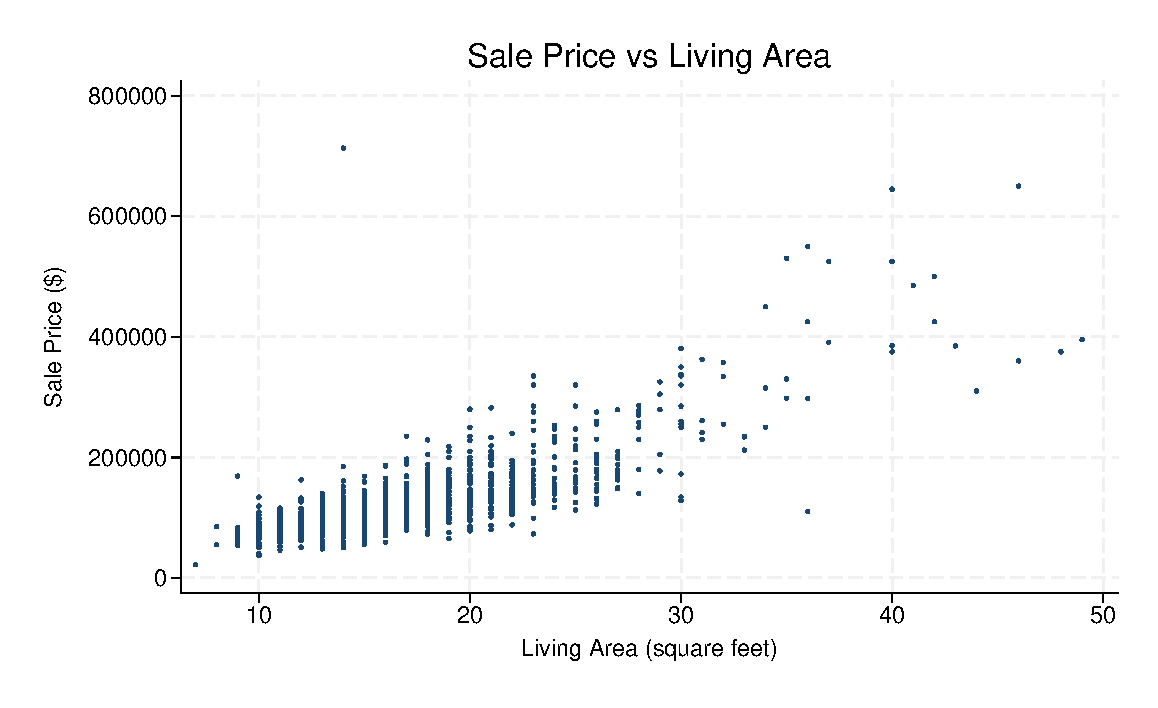
\includegraphics[width=0.81\textwidth]{Figures/0205-scatter_basic.eps}
\caption{Precio de venta de las casas vs área habitable}
\label{fig:0205-scatter_basic}
\end{figure}

\subsubsection*{Salida de Stata de la parte a)}

%\lstinputlisting[label=lst:hwrk-0205-a]{Outputs/ecnm-2502-outp-hwrk-0201-a.txt}

\subsection*{b) Modelo de Regresión Lineal de las casas}
\subsubsection*{Salida de Stata de la parte b)}

\subsubsection*{Ecuación Estimada}
El modelo de regresión lineal estimado es:
\[
\widehat{sprice} = -30,069.2 + 9,181.71 \cdot livarea
\]
\begin{align}
\text{Error estándar:} \quad & (3,211.57) \quad (182.33) \\
\text{Estadístico t:} \quad & (-9.36) \quad\quad (50.36) \\
\end{align}

\subsubsection*{Interpretación de las Estimaciones}

\textbf{Coeficiente de pendiente ($\hat{\beta}_1 = 9,181.71$):}
\begin{itemize}
    \item Por cada pie cuadrado adicional de área habitable, el precio de venta aumenta en promedio \$9,181.71, manteniendo todo lo demás constante.
    \item Este coeficiente es altamente significativo (t = 50.36, p < 0.001), con un intervalo de confianza al 95\% de [\$8,824.07, \$9,539.36].
    \item La fuerte significancia estadística indica una relación positiva muy robusta entre el área habitable y el precio de venta.
\end{itemize}

\textbf{Intercepto ($\hat{\beta}_0 = -30,069.2$):}
\begin{itemize}
    \item El intercepto negativo sugiere que una casa hipotética con 0 pies cuadrados tendría un precio de -\$30,069.2.
    \item Este valor no tiene interpretación práctica, pues no existen casas con área cero. El intercepto solo sirve en este caso para ajustar la línea de regresión.
    \item Es estadísticamente significativo (t = -9.36, p < 0.001).
\end{itemize}

\subsubsection*{Boceto de la Línea Ajustada}

\subsection*{c) Modelo Cuadrático}

\subsubsection*{Salida de Stata de la parte c)}

\subsubsection*{Ecuación Estimada}
El modelo cuadrático estimado es:
\[
\widehat{sprice} = 57,728.31 + 212.611 \cdot livarea^2
\]
\begin{align}
\text{Error estándar:} \quad & (1,546.67) \quad (3.932) \\
\text{Estadístico t:} \quad & (37.32) \quad\quad (54.08) \\
\end{align}

\subsubsection*{Interpretación de las Estimaciones}

\textbf{Coeficiente de $livarea^2$ ($\hat{\beta}_1 = 212.611$):}
\begin{itemize}
    \item Este coeficiente indica que el precio aumenta de forma cuadrática con el área habitable.
    \item Es altamente significativo (t = 54.08, p < 0.001), con un intervalo de confianza al 95\% de [204.90, 220.32].
    \item El modelo cuadrático implica que el efecto marginal del área habitable sobre el precio no es constante, sino que aumenta con el tamaño de la casa.
\end{itemize}

\textbf{Intercepto ($\hat{\beta}_0 = 57,728.31$):}
\begin{itemize}
    \item Representa el precio predicho cuando el área habitable es cero.
    \item A diferencia del modelo lineal, este intercepto es positivo (\$57,728.31).
    \item Es estadísticamente significativo (t = 37.32, p < 0.001).
\end{itemize}

\subsubsection*{Efecto Marginal en una Casa de 1,500 Pies Cuadrados}

Para calcular el efecto marginal, se deriva la función de precio con respecto al área habitable:
\[
\frac{\partial sprice}{\partial livarea} = \frac{\partial}{\partial livarea}(\beta_0 + \beta_1 \cdot livarea^2) = 2\beta_1 \cdot livarea
\]

Se evalúa en $livarea = 1,500$ pies cuadrados:
\[
\frac{\partial sprice}{\partial livarea}\bigg|_{livarea=1,500} = 2 \times 212.611 \times 1,500 = 637,833
\]

\textbf{Interpretación del efecto marginal:}
\begin{itemize}
    \item En una casa con 1,500 pies cuadrados, cada pie cuadrado adicional aumenta el precio en \$637.83.
    \item Por lo tanto, 100 pies cuadrados adicionales aumentarían el precio en aproximadamente:
    \[
    \Delta sprice \approx 637.83 \times 100 = \boxed{\$63,783}
    \]
\end{itemize}

\subsection*{d) Comparación Gráfica y Numérica de los Modelos}

\subsubsection*{Gráfico Comparativo de las Líneas Ajustadas}

La Figura \ref{fig:fitted_comparison} muestra la nube de puntos de los precios de venta versus el área habitable, junto con las líneas ajustadas de ambos modelos.

\begin{figure}[htbp]
    \centering
    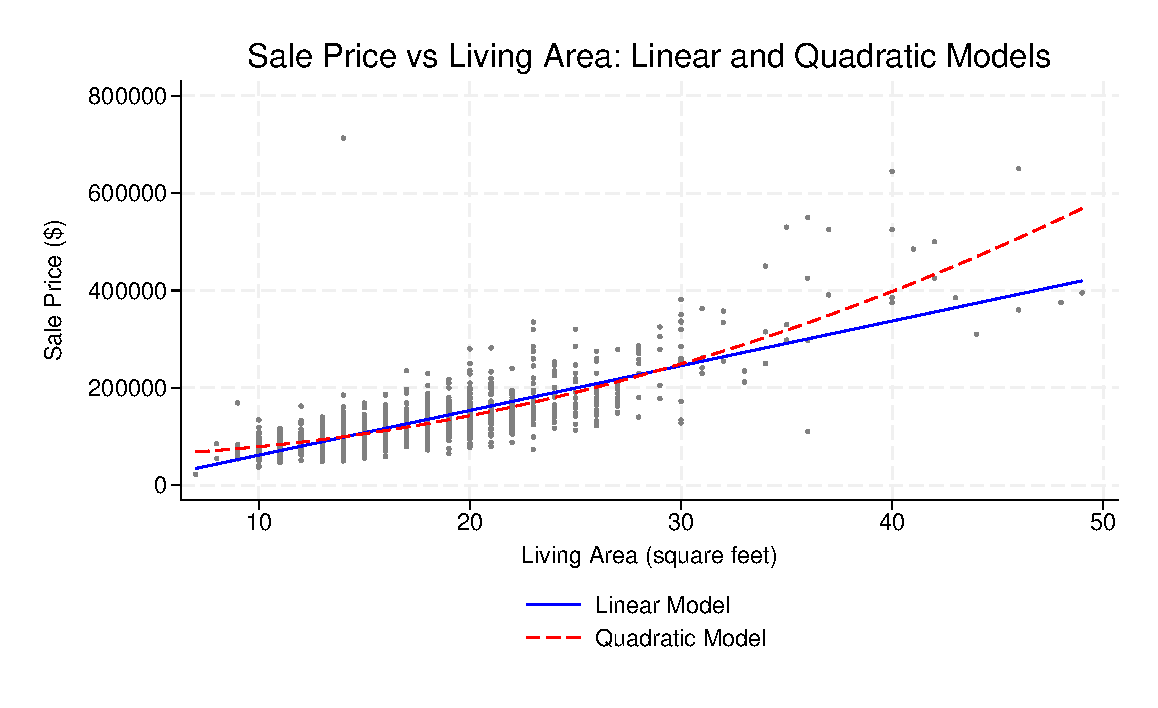
\includegraphics[width=0.85\textwidth]{Figures/0205-fitted_comparison.eps}
    \caption{Precio de Venta vs Área Habitable: Comparación de Modelos Lineal y Cuadrático}
    \label{fig:fitted_comparison}
\end{figure}

\subsubsection*{Análisis Visual del Ajuste}

Al examinar el gráfico, se observan las siguientes características:

\begin{enumerate}
    \item \textbf{Modelo Lineal:} 
    \begin{itemize}
        \item Presenta una relación constante entre área habitable y precio.
        \item La pendiente es uniforme a lo largo de todo el rango de datos.
        \item Parece subestimar los precios para casas muy pequeñas (menos de 1,000 pies²).
        \item También subestima los precios para casas muy grandes (más de 3,000 pies²).
        \item Tiende a sobreestimar los precios en el rango medio (1,500-2,000 pies²).
    \end{itemize}
    
    \item \textbf{Modelo Cuadrático:}
    \begin{itemize}
        \item Muestra una relación no lineal, con curvatura convexa.
        \item El efecto marginal del área habitable aumenta con el tamaño de la casa.
        \item Se ajusta mejor a la tendencia de los datos en los extremos del rango.
        \item Captura mejor la aceleración del precio para casas grandes.
        \item Proporciona un mejor ajuste visual a la nube de puntos.
    \end{itemize}
\end{enumerate}

\subsection*{Comparación de la Suma de Errores al Cuadrado (SSE)}

\begin{table}[h]
\centering
\begin{tabular}{lcc}
\hline
\textbf{Modelo} & \textbf{SSE} & \textbf{Diferencia con Cuadrático} \\
\hline
Lineal & $2.227 \times 10^{12}$ & $+1.955 \times 10^{11}$ \\
Cuadrático & $2.031 \times 10^{12}$ & --- \\
\hline
\end{tabular}
\caption{Comparación de SSE entre modelos}
\label{tab:sse_comparison}
\end{table}

\textbf{Análisis de SSE:}
\begin{itemize}
    \item El modelo cuadrático tiene menor SSE ($2.031 \times 10^{12}$) que el modelo lineal ($2.227 \times 10^{12}$).
    \item La diferencia en SSE es de $1.955 \times 10^{11}$ dólares al cuadrado.
    \item Esta reducción en SSE representa una mejora del $\frac{1.955 \times 10^{11}}{2.227 \times 10^{12}} \times 100 = 8.78\%$ en el ajuste.
    \item La menor SSE del modelo cuadrático indica que produce errores de predicción más pequeños en promedio.
\end{itemize}

\subsection*{Conclusiones}

\begin{enumerate}
    \item \textbf{¿Cuál parece ajustarse mejor a los datos?}
    
    El \textbf{modelo cuadrático} parece ajustarse mejor a los datos tanto visual como numéricamente. Visualmente, la línea cuadrática sigue más fielmente la tendencia no lineal de la nube de puntos, especialmente en los extremos del rango de área habitable.
    
    \item \textbf{¿Cuál modelo tiene menor SSE?}
    
    El \textbf{modelo cuadrático tiene menor SSE} ($2.031 \times 10^{12}$ vs $2.227 \times 10^{12}$), lo que confirma cuantitativamente la impresión visual de un mejor ajuste.
    
\end{enumerate}

\subsection*{e) Modelo Cuadrático por Tipo de Lote}

\subsubsection*{Salida de Stata de la parte e)}

\subsubsection*{Distribución de la Muestra}

Antes de analizar los modelos, se debe notar la distribución de los tipos de lotes:
\begin{itemize}
    \item \textbf{Lotes grandes} (>0.5 acres): 95 casas (6.33\% de la muestra)
    \item \textbf{Lotes no grandes} (≤0.5 acres): 1,405 casas (93.67\% de la muestra)
\end{itemize}

Las casas en lotes grandes tienen características notablemente diferentes:
\begin{itemize}
    \item Precio medio: \$249,017 (lotes grandes) vs \$115,220 (lotes no grandes)
    \item Área habitable media: 2,463 pies² (lotes grandes) vs 1,621 pies² (lotes no grandes)
\end{itemize}

\subsubsection*{Modelos estimados}

\textbf{1. Modelo para Lotes Grandes (n = 95):}
\[
\widehat{sprice} = 113,279.4 + 193.83 \cdot livarea^2
\]
\begin{align}
\text{Error estándar:} \quad & (12,824.6) \quad (14.62) \\
\text{Estadístico t:} \quad & (8.83) \quad\quad (13.26) \\
R^2 = 0.654, \quad & RMSE = \$75,251
\end{align}

\textbf{2. Modelo para Lotes No Grandes (n = 1,405):}
\[
\widehat{sprice} = 62,172.4 + 186.86 \cdot livarea^2
\]
\begin{align}
\text{Error estándar:} \quad & (1,503.1) \quad (4.47) \\
\text{Estadístico t:} \quad & (41.36) \quad (41.83) \\
R^2 = 0.555, \quad & RMSE = \$30,238
\end{align}

\subsubsection*{Interpretación de las Estimaciones}

\textbf{Coeficientes de $livarea^2$}

\begin{enumerate}
    \item \textbf{Lotes grandes ($\hat{\beta}_1 = 193.83$):}
    \begin{itemize}
        \item El precio aumenta \$193.83 por cada unidad de área habitable al cuadrado.
        \item Efecto marginal en 1,500 pies²: \$581.49 por pie² adicional.
        \item 100 pies² adicionales aumentan el precio en \$58,149.
    \end{itemize}
    
    \item \textbf{Lotes no grandes ($\hat{\beta}_1 = 186.86$):}
    \begin{itemize}
        \item El precio aumenta \$186.86 por cada unidad de área habitable al cuadrado.
        \item Efecto marginal en 1,500 pies²: \$560.58 por pie² adicional.
        \item 100 pies² adicionales aumentan el precio en \$56,058.
    \end{itemize}
\end{enumerate}

\textbf{Interceptos}

\begin{itemize}
    \item \textbf{Lotes grandes:} \$113,279 - sustancialmente mayor que los lotes no grandes.
    \item \textbf{Lotes no grandes:} \$62,172 - casi la mitad del intercepto para lotes grandes.
    \item Esta diferencia de \$51,107 refleja el valor premium de los lotes grandes, independientemente del área habitable.
\end{itemize}

\subsubsection*{Comparación de Resultados}

\begin{table}[h]
\centering
\begin{tabular}{lcc}
\hline
\textbf{Característica} & \textbf{Lotes Grandes} & \textbf{Lotes No Grandes} \\
\hline
Coeficiente $livarea^2$ & 193.83*** & 186.86*** \\
Error estándar & (14.62) & (4.47) \\
Intercepto & \$113,279*** & \$62,172*** \\
Error estándar & (12,825) & (1,503) \\
\hline
$R^2$ & 0.654 & 0.555 \\
RMSE & \$75,251 & \$30,238 \\
N & 95 & 1,405 \\
SSE & $5.27 \times 10^{11}$ & $1.28 \times 10^{12}$ \\
\hline
Efecto marginal (1,500 pies²) & \$581/pie² & \$561/pie² \\
Efecto de 100 pies² adicionales & \$58,149 & \$56,058 \\
\hline
\end{tabular}
\caption{Comparación del Modelo Cuadrático por Tipo de Lote}
\label{tab:lots_comparison}
\end{table}

\begin{figure}[htbp]
    \centering
    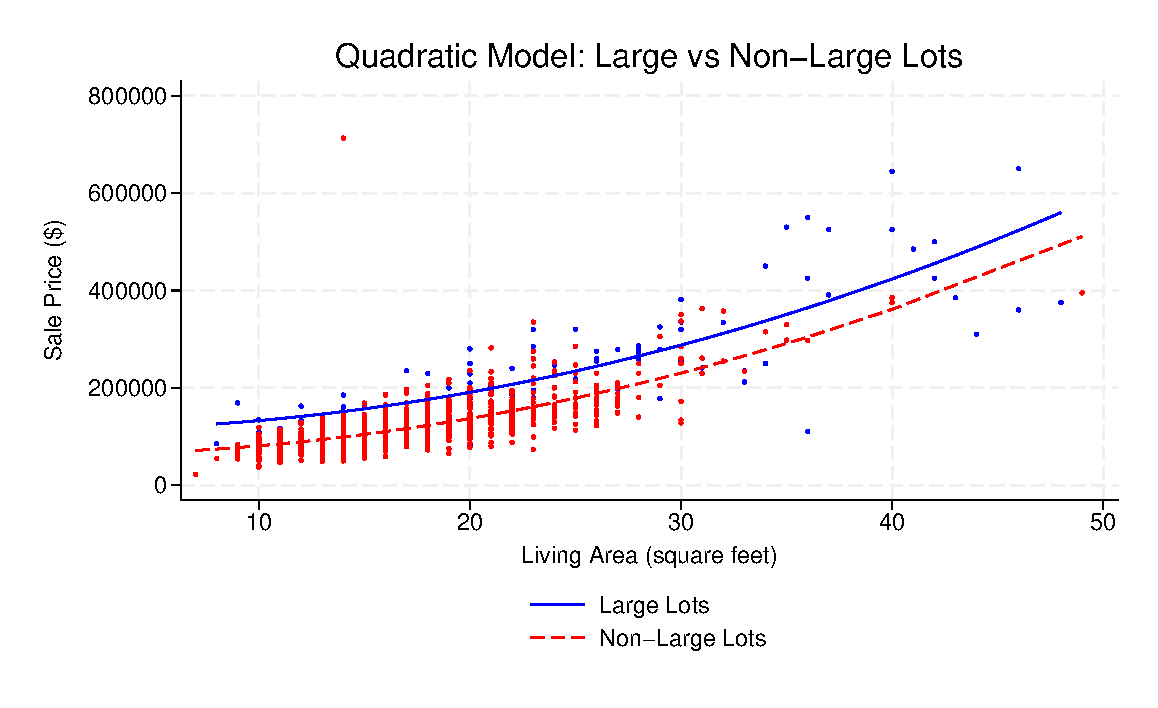
\includegraphics[width=0.85\textwidth]{Figures/0205-lots_comparison.eps}
    \caption{Modelo Cuadrático: Comparación entre Lotes Grandes y No Grandes}
    \label{fig:lots_comparison}
\end{figure}

\subsection*{Conclusiones}

\begin{enumerate}
    \item \textbf{Similitudes:}
    \begin{itemize}
        \item Ambos modelos muestran una relación cuadrática significativa entre área y precio.
        \item Los coeficientes de $livarea^2$ son similares (193.83 vs 186.86) y la diferencia no es estadísticamente significativa.
        \item Ambos tienen buen poder explicativo, aunque el $R^2$ es mayor para lotes grandes.
    \end{itemize}
    
    \item \textbf{Diferencias principales:}
    \begin{itemize}
        \item El \textbf{intercepto es 82\% mayor} para lotes grandes (\$113,279 vs \$62,172), reflejando un premium sustancial.
        \item El \textbf{RMSE es mayor} para lotes grandes (\$75,251 vs \$30,238), indicando mayor variabilidad en precios.
        \item El \textbf{$R^2$ es mayor} para lotes grandes (0.654 vs 0.555), sugiriendo que el área habitable explica mejor el precio en este segmento.
    \end{itemize}
    
\end{enumerate}

\subsection*{f) Modelos con la Edad de la Casa}

\subsubsection*{Salida de Stata de la parte f)}

\subsubsection*{Análisis Gráfico Inicial}

La Figura \ref{fig:price_age_scatter} muestra la relación entre el precio de venta y la edad de la casa.

\begin{figure}[htbp]
    \centering
    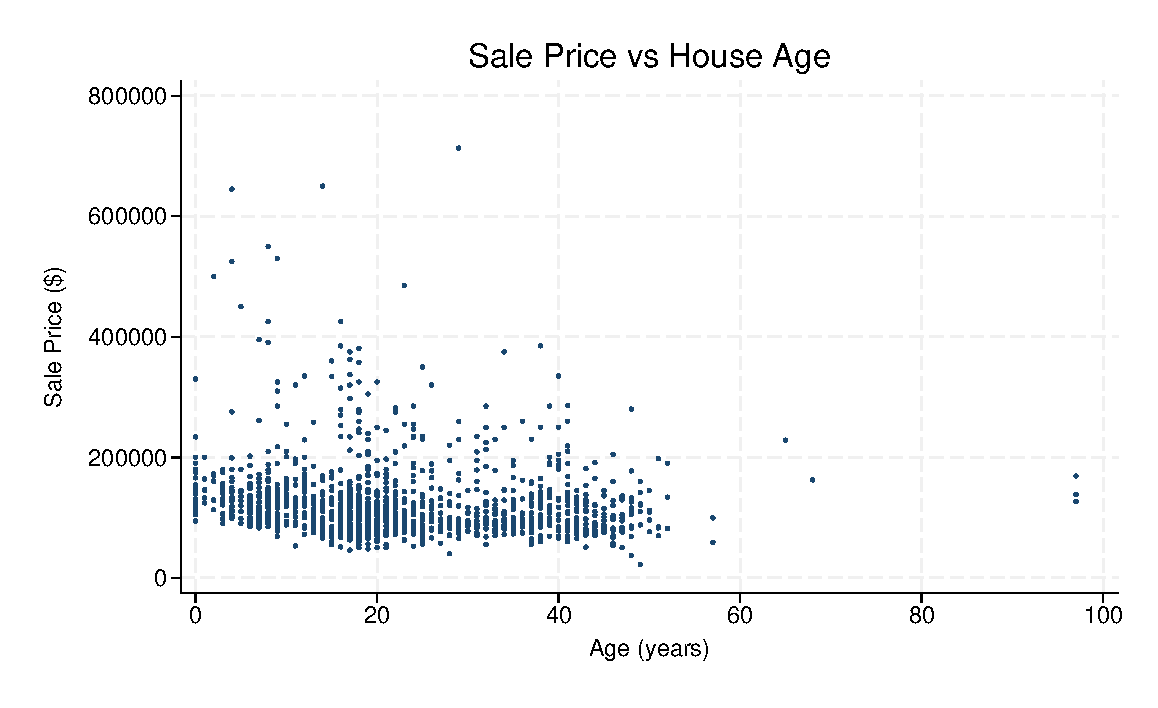
\includegraphics[width=0.8\textwidth]{Figures/0205-price_age_scatter.eps}
    \caption{Precio de Venta vs Edad de la Casa}
    \label{fig:price_age_scatter}
\end{figure}

\textbf{Observaciones del gráfico de dispersión:}
\begin{itemize}
    \item Alta dispersión en los precios para todas las edades.
    \item Tendencia negativa débil entre edad y precio.
    \item Gran variabilidad, especialmente para casas nuevas (0-10 años).
    \item Presencia de valores atípicos en todas las edades.
\end{itemize}

\subsubsection*{Modelo Lineal}

\[
\widehat{sprice} = 137,403.6 - 627.16 \cdot age
\]
\begin{align}
\text{Error estándar:} \quad & (3,149.3) \quad (123.6) \\
\text{Estadístico t:} \quad & (43.63) \quad (-5.08) \\
\text{p-valor:} \quad & (0.000) \quad (0.000)
\end{align}

\textbf{Interpretación de Coeficientes}

\begin{itemize}
    \item \textbf{Intercepto ($\hat{\beta}_0 = 137,403.6$):}
    \begin{itemize}
        \item Representa el precio predicho de una casa nueva (edad = 0).
        \item Una casa nueva tiene un precio esperado de \$137,404.
        \item Es altamente significativo (t = 43.63, p < 0.001).
    \end{itemize}
    
    \item \textbf{Coeficiente de edad ($\hat{\beta}_1 = -627.16$):}
    \begin{itemize}
        \item Por cada año adicional de edad, el precio disminuye en promedio \$627.16.
        \item Es estadísticamente significativo (t = -5.08, p < 0.001).
        \item Intervalo de confianza al 95\%: [-869.52, -384.81].
        \item Una casa de 20 años vale aproximadamente \$12,543 menos que una casa nueva.
        \item Una casa de 50 años vale aproximadamente \$31,358 menos que una casa nueva.
    \end{itemize}
\end{itemize}

\subsubsection*{Modelo Log-Lineal}

\[
\widehat{\ln(sprice)} = 11.746 - 0.00476 \cdot age
\]
\begin{align}
\text{Error estándar:} \quad & (0.0188) \quad (0.0007) \\
\text{Estadístico t:} \quad & (623.26) \quad (-6.44) \\
\text{p-valor:} \quad & (0.000) \quad (0.000)
\end{align}

\textbf*{Interpretación de Coeficientes}

\begin{itemize}
    \item \textbf{Intercepto ($\hat{\beta}_0 = 11.746$):}
    \begin{itemize}
        \item $\ln(sprice)$ para una casa nueva (edad = 0).
        \item Implica un precio esperado de $e^{11.746} = \$126,684$ para una casa nueva.
    \end{itemize}
    
    \item \textbf{Coeficiente de edad ($\hat{\beta}_1 = -0.00476$):}
    \begin{itemize}
        \item Cada año adicional de edad reduce el precio en aproximadamente \textbf{0.476\%}.
        \item Es estadísticamente significativo (t = -6.44, p < 0.001).
        \item La depreciación es proporcional al valor de la casa.
        \item Una casa de 20 años vale aproximadamente $20 \times 0.476\% = 9.52\%$ menos.
        \item Una casa de 50 años vale aproximadamente $50 \times 0.476\% = 23.8\%$ menos.
    \end{itemize}
\end{itemize}

\subsubsection*{Comparación Visual de los Modelos}

\begin{figure}[htbp]
    \centering
    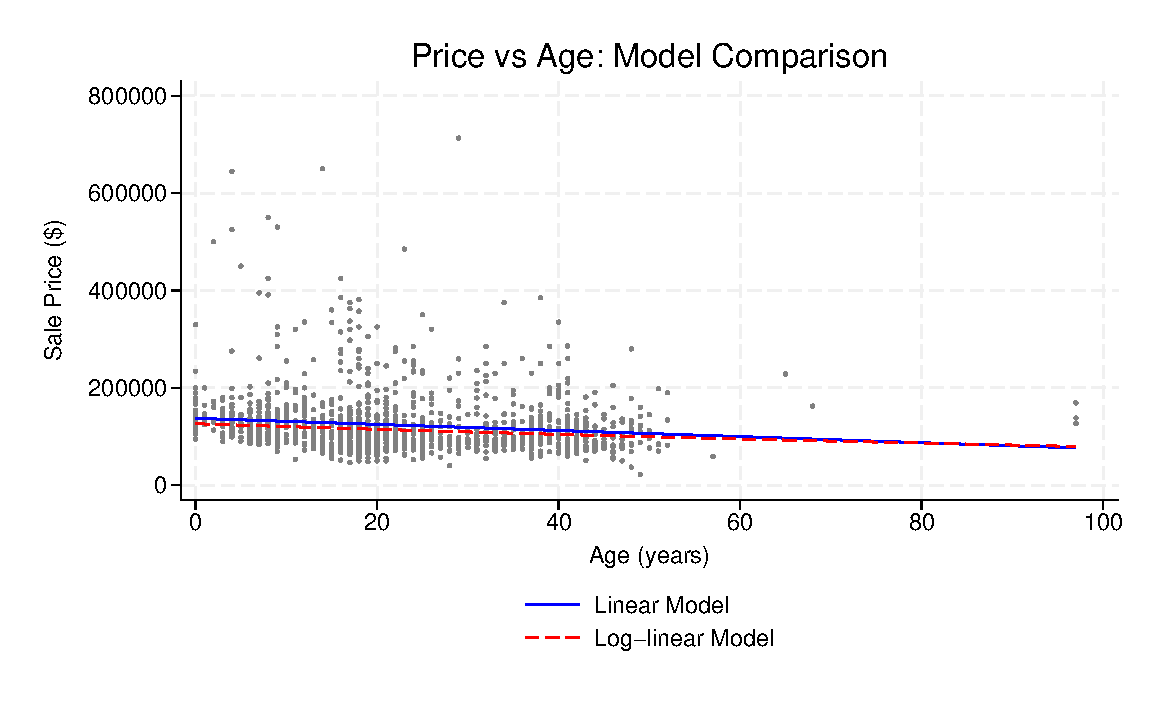
\includegraphics[width=0.85\textwidth]{Figures/0205-age_models_comparison.eps}
    \caption{Comparación de Modelos: Lineal vs Log-lineal}
    \label{fig:age_models_comparison}
\end{figure}

\subsubsection*{Comparación Cuantitativa}

\begin{table}[h]
\centering
\begin{tabular}{lcc}
\hline
\textbf{Criterio} & \textbf{Modelo Lineal} & \textbf{Modelo Log-lineal} \\
\hline
$R^2$ & 0.0169 & 0.0269 \\
$R^2$ ajustado & 0.0163 & 0.0263 \\
RMSE & \$62,735 & 0.3754* \\
AIC & 37,400 & 1,320 \\
BIC & 37,400 & 1,330 \\
\hline
Depreciación anual & \$627 constante & 0.476\% del valor \\
Depreciación a 20 años & \$12,543 & 9.52\% del valor \\
Depreciación a 50 años & \$31,358 & 23.8\% del valor \\
\hline
\end{tabular}
\caption{Comparación de Modelos de Edad. *RMSE del modelo log-lineal está en escala logarítmica}
\label{tab:age_comparison}
\end{table}

\subsubsection*{¿Cuál Modelo Preferir?}

Basándose en el análisis gráfico y estadístico, \textbf{preferiría el modelo log-lineal} por las siguientes razones:

\begin{enumerate}
    
    \item \textbf{Interpretación económica más realista:}
    \begin{itemize}
        \item El modelo log-lineal implica depreciación \textbf{porcentual constante} (0.476\% anual).
        \item El modelo lineal implica depreciación \textbf{absoluta constante} (\$627 anual).
        \item La depreciación porcentual es más coherente con la teoría económica: una casa de \$500,000 debería depreciarse más en términos absolutos que una de \$100,000.
    \end{itemize}
    
    \item \textbf{Comportamiento en los extremos:}
    \begin{itemize}
        \item El modelo lineal puede predecir precios negativos para casas muy viejas (>219 años).
        \item El modelo log-lineal siempre predice precios positivos (asintóticamente hacia cero).
    \end{itemize}
    
    \item \textbf{Ajuste visual:}
    \begin{itemize}
        \item Aunque ambas líneas son similares en el rango observado, el modelo log-lineal muestra una ligera curvatura que se ajusta mejor a la tendencia de los datos.
        \item La curvatura convexa del modelo log-lineal captura mejor la mayor dispersión en casas nuevas.
    \end{itemize}
\end{enumerate}

\end{document}
